% Options for packages loaded elsewhere
\PassOptionsToPackage{unicode}{hyperref}
\PassOptionsToPackage{hyphens}{url}
%
\documentclass[
]{article}
\usepackage{amsmath,amssymb}
\usepackage{stata}
\usepackage{iftex}
\ifPDFTeX
  \usepackage[T1]{fontenc}
  \usepackage[utf8]{inputenc}
  \usepackage{textcomp} % provide euro and other symbols
\else % if luatex or xetex
  \usepackage{unicode-math} % this also loads fontspec
  \defaultfontfeatures{Scale=MatchLowercase}
  \defaultfontfeatures[\rmfamily]{Ligatures=TeX,Scale=1}
\fi
\usepackage{lmodern}
\ifPDFTeX\else
  % xetex/luatex font selection
\fi
% Use upquote if available, for straight quotes in verbatim environments
\IfFileExists{upquote.sty}{\usepackage{upquote}}{}
\IfFileExists{microtype.sty}{% use microtype if available
  \usepackage[]{microtype}
  \UseMicrotypeSet[protrusion]{basicmath} % disable protrusion for tt fonts
}{}
\makeatletter
\@ifundefined{KOMAClassName}{% if non-KOMA class
  \IfFileExists{parskip.sty}{%
    \usepackage{parskip}
  }{% else
    \setlength{\parindent}{0pt}
    \setlength{\parskip}{6pt plus 2pt minus 1pt}}
}{% if KOMA class
  \KOMAoptions{parskip=half}}
\makeatother
\usepackage{xcolor}
\usepackage[margin=1 in]{geometry}
\usepackage{longtable,booktabs,array}
\usepackage{calc} % for calculating minipage widths
% Correct order of tables after \paragraph or \subparagraph
\usepackage{etoolbox}
\makeatletter
\patchcmd\longtable{\par}{\if@noskipsec\mbox{}\fi\par}{}{}
\makeatother
% Allow footnotes in longtable head/foot
\IfFileExists{footnotehyper.sty}{\usepackage{footnotehyper}}{\usepackage{footnote}}
\makesavenoteenv{longtable}
\usepackage{graphicx}
\makeatletter
\def\maxwidth{\ifdim\Gin@nat@width>\linewidth\linewidth\else\Gin@nat@width\fi}
\def\maxheight{\ifdim\Gin@nat@height>\textheight\textheight\else\Gin@nat@height\fi}
\makeatother
% Scale images if necessary, so that they will not overflow the page
% margins by default, and it is still possible to overwrite the defaults
% using explicit options in \includegraphics[width, height, ...]{}
\setkeys{Gin}{width=\maxwidth,height=\maxheight,keepaspectratio}
% Set default figure placement to htbp
\makeatletter
\def\fps@figure{htbp}
\makeatother
\setlength{\emergencystretch}{3em} % prevent overfull lines
\providecommand{\tightlist}{%
  \setlength{\itemsep}{0pt}\setlength{\parskip}{0pt}}
\setcounter{secnumdepth}{-\maxdimen} % remove section numbering
\ifLuaTeX
  \usepackage{selnolig}  % disable illegal ligatures
\fi
\usepackage{bookmark}
\IfFileExists{xurl.sty}{\usepackage{xurl}}{} % add URL line breaks if available
\urlstyle{same}
\hypersetup{
  pdftitle={Installing and Using the Michigan Graph Scheme},
  pdfauthor={Andy Grogan-Kaylor},
  hidelinks,
  pdfcreator={LaTeX via pandoc}}

\title{Installing and Using the Michigan Graph Scheme}
\author{Andy Grogan-Kaylor}
\date{16 Feb 2025 13:03:12}

\begin{document}
\maketitle

\section{Introduction}\label{introduction}



\begin{figure}
\centering
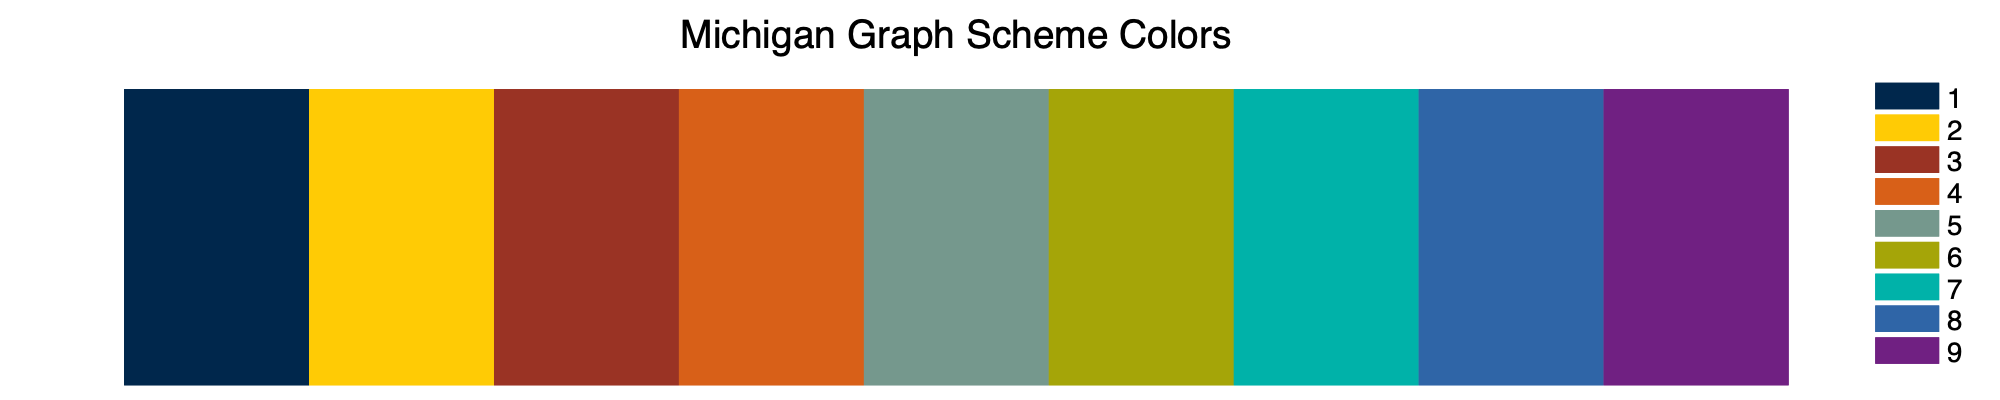
\includegraphics[width=0.75\textwidth,height=\textheight]{MichiganColorsStata.png}
\caption{Colors in Michigan Graph Scheme}
\end{figure}

Stata provides the use of graph schemes that improve the overall look of
graphs.

See \texttt{help\ scheme}.

The \emph{Michigan graph scheme} makes use of official University of
Michigan colors.

\section{Installation}\label{installation}

Use of the \emph{Michigan graph scheme} depends on installation of the
\texttt{lean2} graph scheme developed by Svend Juul.

Type \texttt{findit\ lean2} and click through on the install links to
install \texttt{lean2}.

Then type \texttt{net\ from\ https://agrogan1.github.io/Stata} and click
the links to install.

\section{Example Data}\label{example-data}

We are going to use the famous ``iris'' data collected by Edgar
Anderson.

\begin{stlog}
. clear all
{\smallskip}
.     
. use "iris.dta", clear
{\smallskip}
. 
. summarize
{\smallskip}
    Variable {\VBAR}        Obs        Mean    Std. dev.       Min        Max
\HLI{13}{\PLUS}\HLI{57}
Sepal_Length {\VBAR}        150    5.843333    .8280661        4.3        7.9
 Sepal_Width {\VBAR}        150    3.057333    .4358663          2        4.4
Petal_Length {\VBAR}        150       3.758    1.765298          1        6.9
 Petal_Width {\VBAR}        150    1.199333    .7622377         .1        2.5
     Species {\VBAR}        150           2    .8192319          1          3
\end{stlog}

\section{Histogram}\label{histogram}

\begin{stlog}
. histogram Petal_Length, scheme(michigan)
(bin=12, start=1, width=.49166667)
\end{stlog}



\begin{figure}
\centering
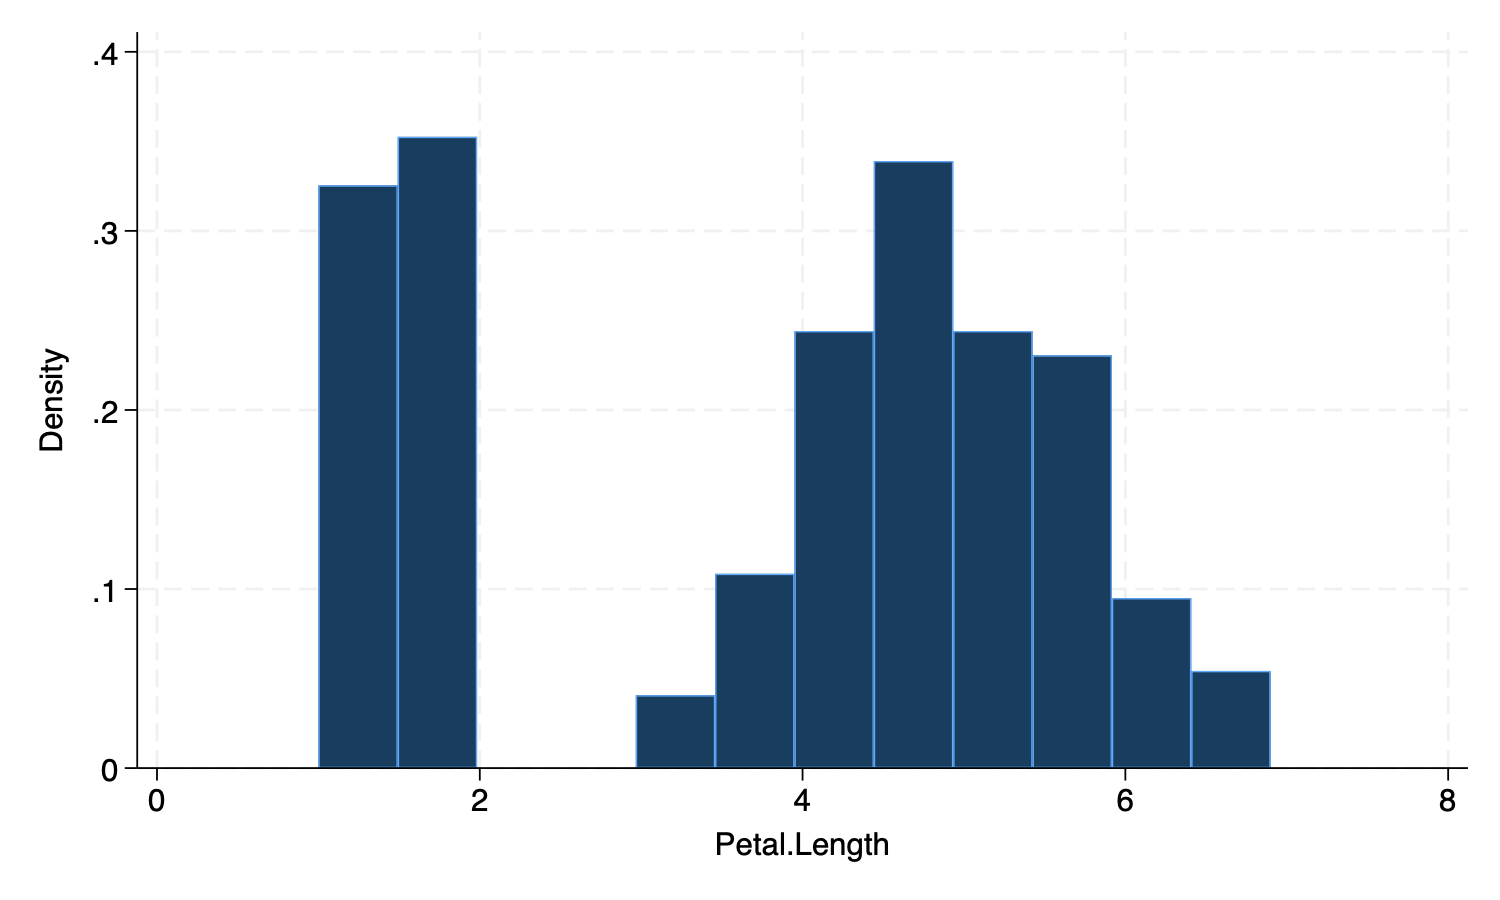
\includegraphics[width=0.5\textwidth,height=\textheight]{myhistogram.png}
\caption{Histogram Using Michigan Scheme}
\end{figure}

\section{Histogram With Transparency}\label{histogram-with-transparency}

\begin{stlog}
. histogram Petal_Length, fcolor(\%50) scheme(michigan)
(bin=12, start=1, width=.49166667)
\end{stlog}



\begin{figure}
\centering
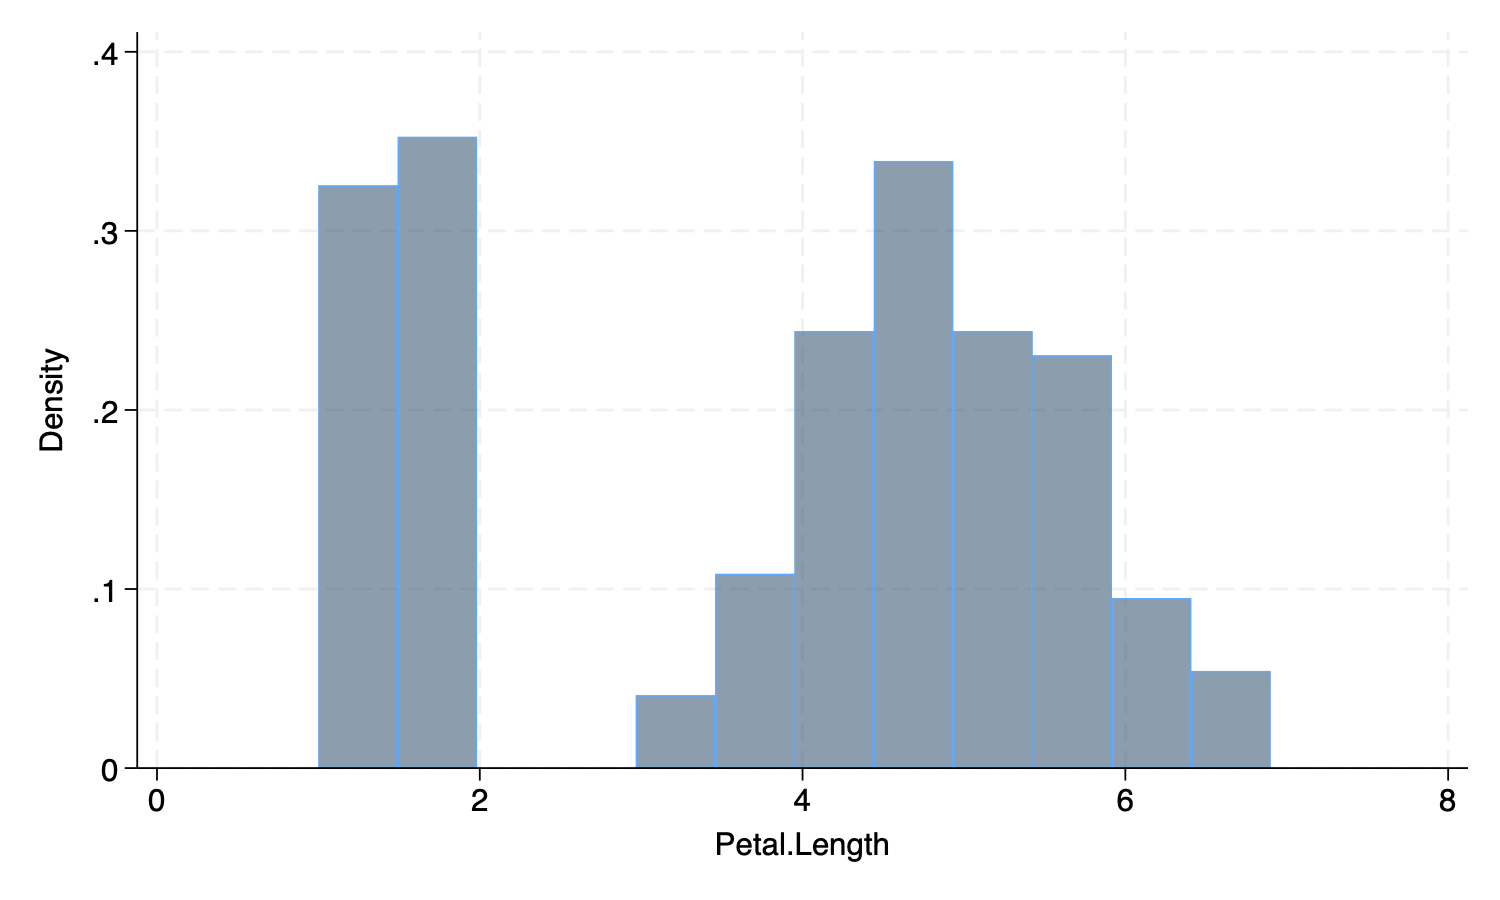
\includegraphics[width=0.5\textwidth,height=\textheight]{myhistogram2.png}
\caption{Histogram Using Michigan Scheme And Slightly Transparent Bars}
\end{figure}

\section{Bar Graph}\label{bar-graph}

\begin{stlog}
. graph bar Petal_Length, over(Species) scheme(michigan) asyvars
\end{stlog}



\begin{figure}
\centering
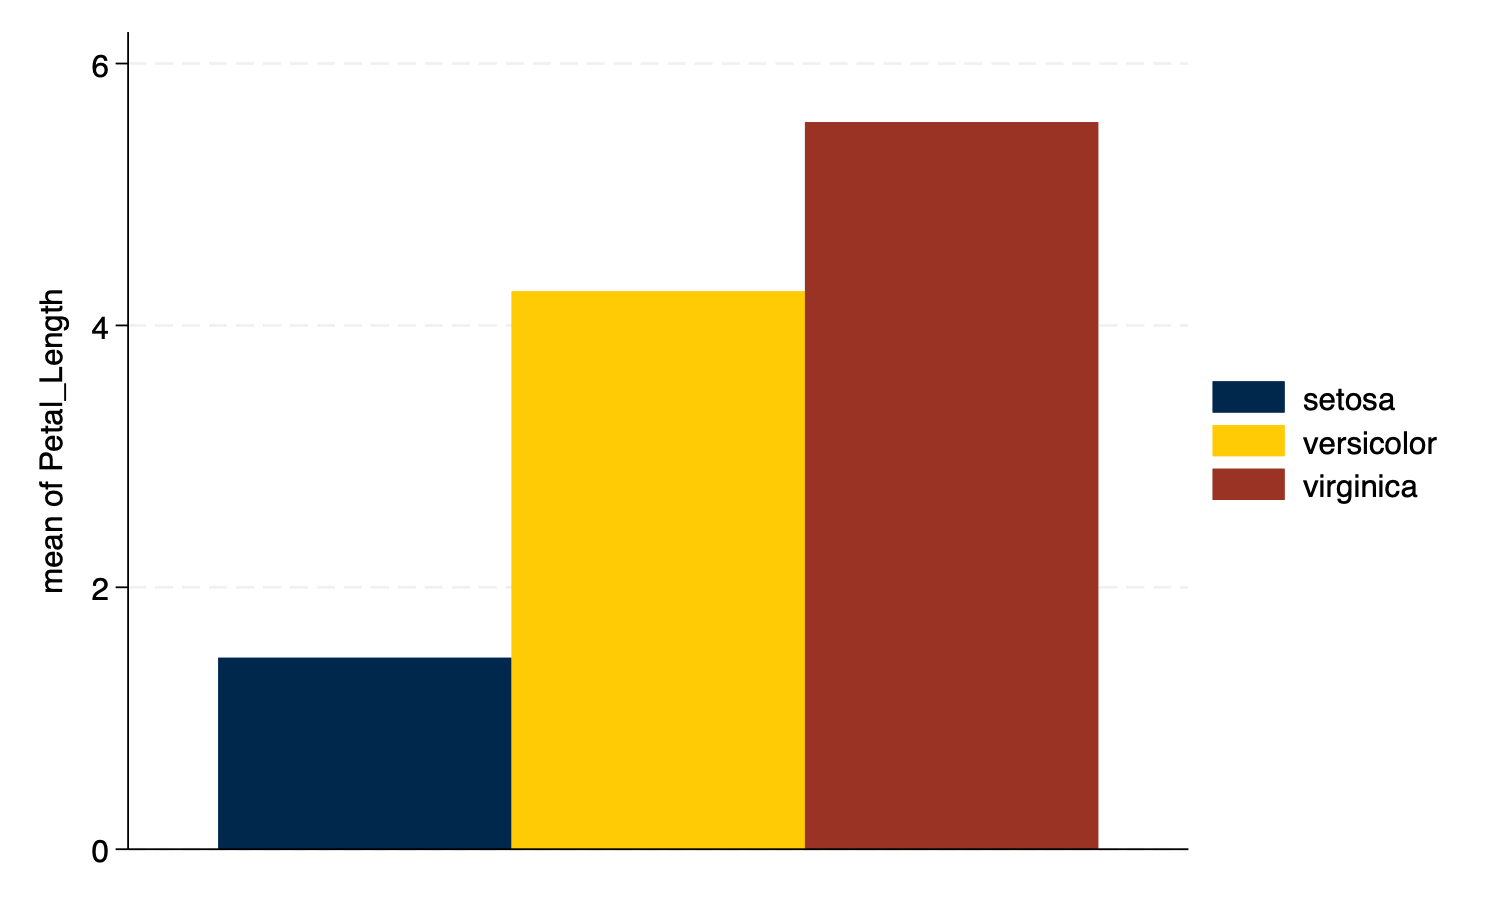
\includegraphics[width=0.5\textwidth,height=\textheight]{mybargraph.png}
\caption{Bar Graph Using Michigan Scheme}
\end{figure}

\section{Bar Graph With Transparency}\label{bar-graph-with-transparency}

\begin{stlog}
. graph bar Petal_Length, over(Species) intensity(70) scheme(michigan) asyvars
\end{stlog}



\begin{figure}
\centering
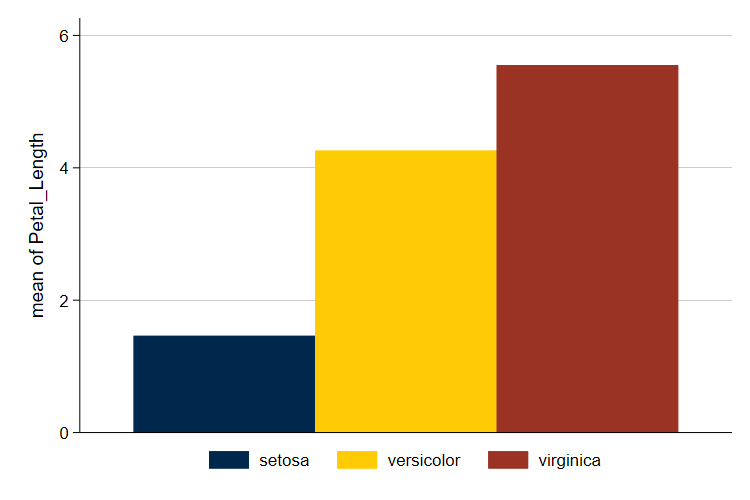
\includegraphics[width=0.5\textwidth,height=\textheight]{mybargraph2.png}
\caption{Bar Graph Using Michigan Scheme and Slightly Transparent Bars}
\end{figure}

\section{Scatterplot}\label{scatterplot}

\begin{stlog}
. twoway (scatter Petal_Length Petal_Width) ///
> (lfit Petal_Length Petal_Width), ///
> scheme(michigan)
\end{stlog}



\begin{figure}
\centering
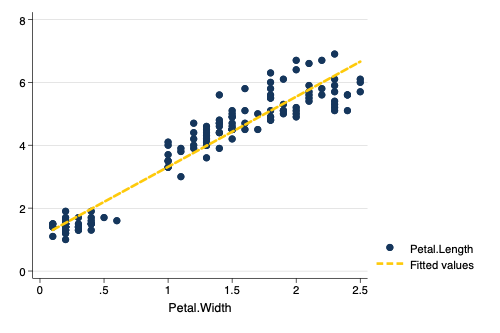
\includegraphics[width=0.5\textwidth,height=\textheight]{myscatter.png}
\caption{Scatterplot Using Michigan Scheme}
\end{figure}

\section{Scatterplot With
Transparency}\label{scatterplot-with-transparency}

\begin{stlog}
. twoway (scatter Petal_Length Petal_Width, mcolor(\%30)) /// markers have 30\% transparency
> (lfit Petal_Length Petal_Width), ///
> scheme(michigan)
\end{stlog}



\begin{figure}
\centering
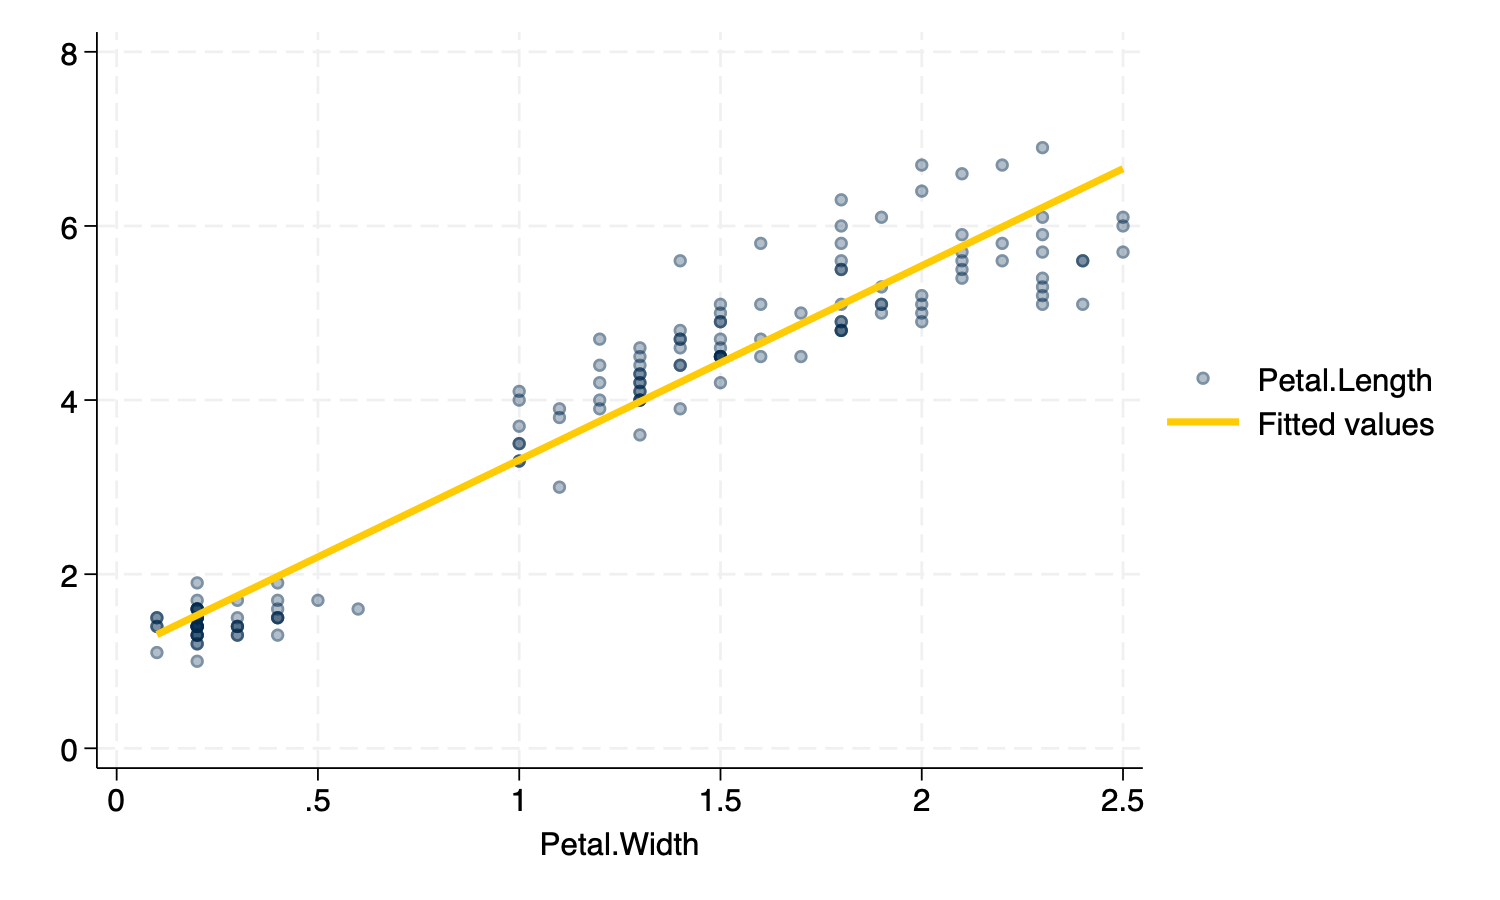
\includegraphics[width=0.5\textwidth,height=\textheight]{myscatter2.png}
\caption{Scatterplot Using Michigan Scheme And Slightly Transparent
Markers}
\end{figure}

\section{Legend Placement}\label{legend-placement}

Sometimes you may wish to have the legend of the graph placed at the
\emph{bottom} of the graph. The \texttt{pos(6)} suboption inside the
\texttt{legend} option will place the legend at the bottom, while you
can manually control the number of legend rows with the \texttt{rows}
suboption.

\begin{stlog}
. graph bar Petal_Length, over(Species) scheme(michigan) asyvars legend(pos(6) rows(1))
\end{stlog}



\begin{figure}
\centering
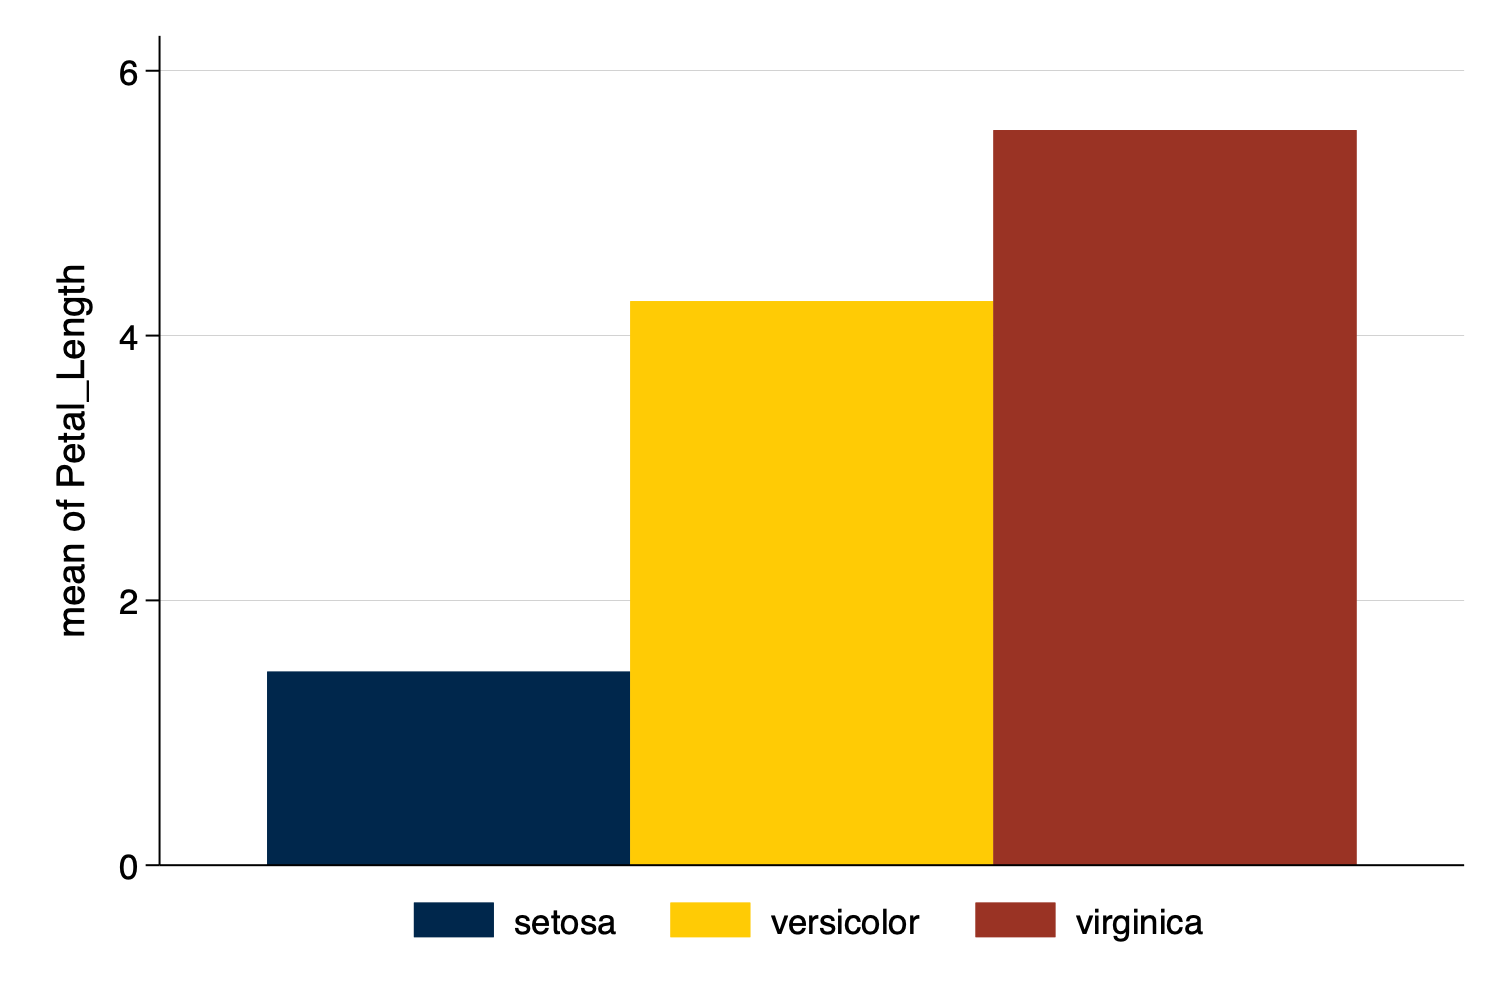
\includegraphics[width=0.5\textwidth,height=\textheight]{mybargraph3.png}
\caption{Bar Graph Using Michigan Scheme and Modified Legend}
\end{figure}

\section{Individual Michigan Colors}\label{individual-michigan-colors}

Individual University of Michigan colors are listed below.

\begin{longtable}[]{@{}
  >{\raggedright\arraybackslash}p{(\columnwidth - 4\tabcolsep) * \real{0.2917}}
  >{\raggedright\arraybackslash}p{(\columnwidth - 4\tabcolsep) * \real{0.1528}}
  >{\raggedright\arraybackslash}p{(\columnwidth - 4\tabcolsep) * \real{0.1528}}@{}}
\toprule\noalign{}
\begin{minipage}[b]{\linewidth}\raggedright
Color
\end{minipage} & \begin{minipage}[b]{\linewidth}\raggedright
Hex
\end{minipage} & \begin{minipage}[b]{\linewidth}\raggedright
RGB
\end{minipage} \\
\midrule\noalign{}
\endhead
\bottomrule\noalign{}
\endlastfoot
Blue & \#00274C & 0 39 76 \\
Maize & \#FFCB05 & 255 203 5 \\
Tappan Red & \#9A3324 & 154 51 36 \\
Ross School Orange & \#D86018 & 216 96 24 \\
Wave Field Green & \#A5A508 & 165 165 8 \\
Taubman Teal & \#00B2A9 & 0 178 169 \\
Arboretum Blue & \#2F65A7 & 47 101 167 \\
Ann Arbor Amethyst & \#702082 & 112 32 130 \\
Matthaei Violet & \#575294 & 87 82 148 \\
Umma Tan & \#CFC096 & 207 192 150 \\
Burton Tower Beige & \#9B9A6D & 155 154 109 \\
Angell Hall Ash & \#989C97 & 152 156 151 \\
Law Quad Stone & \#655A52 & 101 90 82 \\
\end{longtable}

Stata can use RGB codes for colors. As an example.

\begin{stlog}
. twoway (scatter Petal_Length Petal_Width, mcolor("112 32 130 \%30")) /// markers are Amethyst with 30\%
>  transparency
> (lfit Petal_Length Petal_Width, lcolor("87 82 148")), /// Violet line
> scheme(michigan)
\end{stlog}



\begin{figure}
\centering
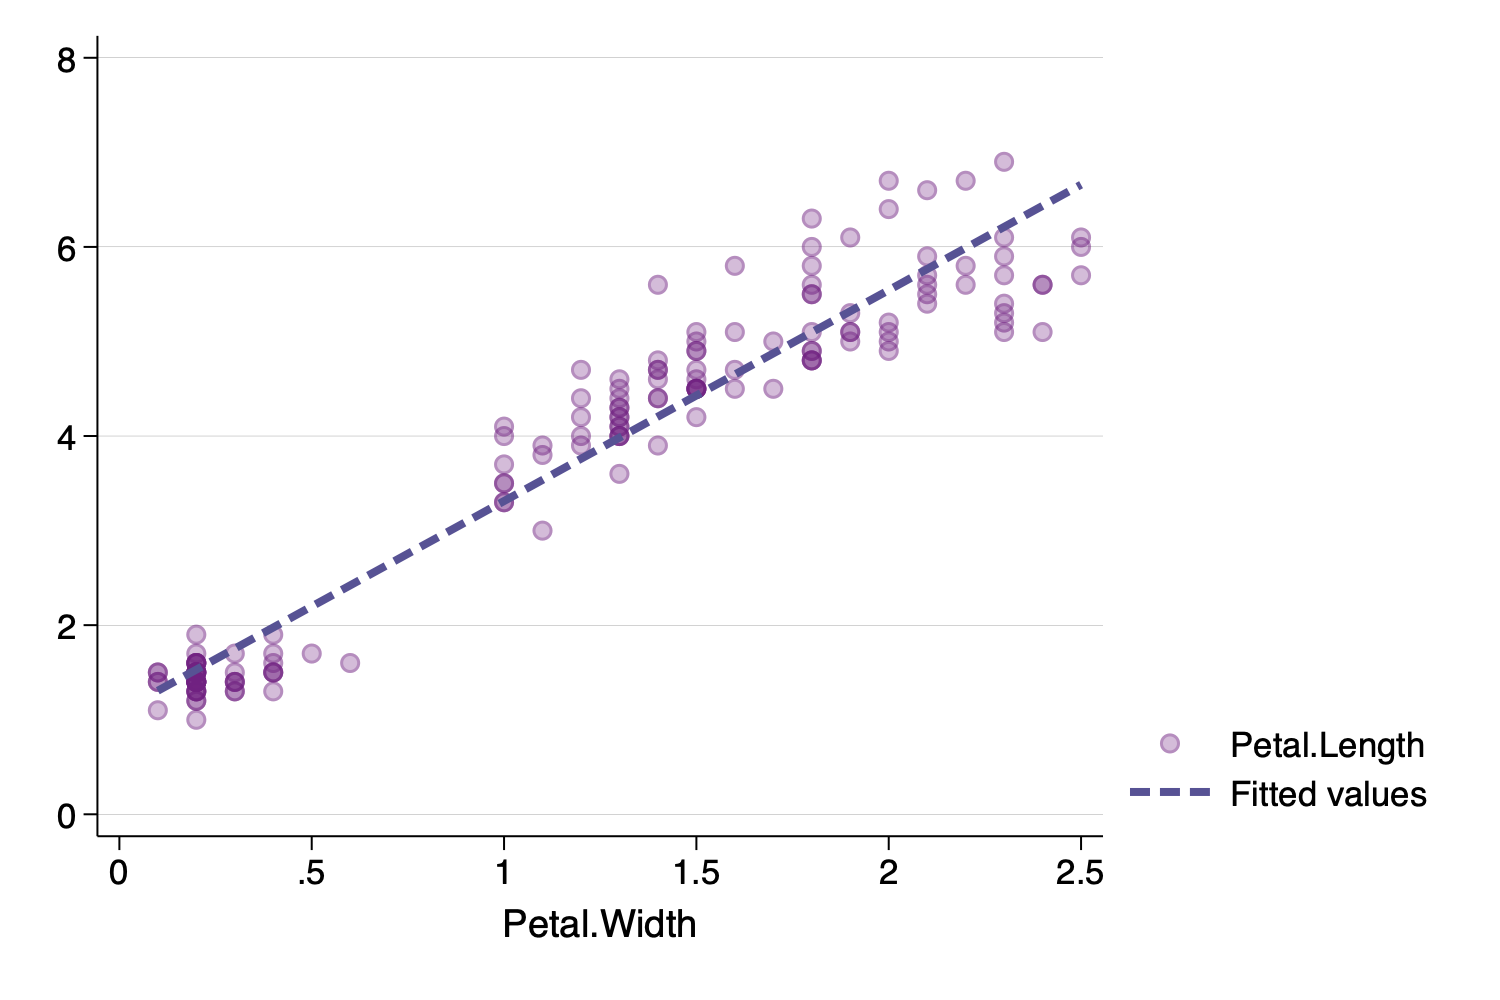
\includegraphics[width=0.5\textwidth,height=\textheight]{myscatter3.png}
\caption{Scatterplot Using Michigan Scheme, Selected Colors, And
Slightly Transparent Markers}
\end{figure}

\newpage

\section{Michigan2 Graph Scheme}\label{michigan2-graph-scheme}

I have also developed a \texttt{michigan2} graph scheme:
\texttt{,\ scheme(michigan2)}.

This graph scheme can be installed using the same instructions as above.
The \texttt{michigan2} scheme slightly reorders the color palette of the
original scheme. The scheme begins with blue and maize, but then moves
to the \emph{cooler} colors before moving to \emph{Tappan Red} and
\emph{Ross Orange}. \emph{Taubman Teal}--a very fluorescent color--is
moved to the end of the palette.



\begin{figure}
\centering
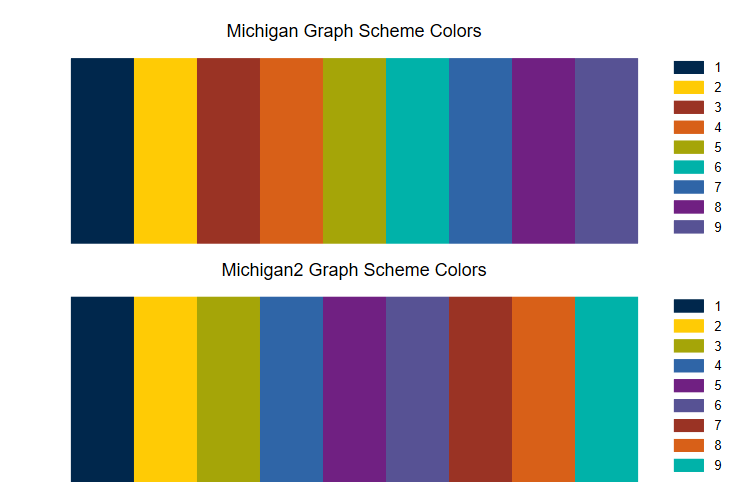
\includegraphics[width=0.5\textwidth,height=\textheight]{MichiganColorsStata3.png}
\caption{Colors in Michigan Graph Schemes}
\end{figure}

\end{document}
